\documentclass[14pt, oneside]{article}   	% use "amsart" instead of "article" for AMSLaTeX format
\usepackage{geometry}                		% See geometry.pdf to learn the layout options. There are lots.
%\geometry{letterpaper}                   		% ... or a4paper or a5paper or ... 
%\geometry{landscape}                		% Activate for for rotated page geometry
%\usepackage[parfill]{parskip}    		% Activate to begin paragraphs with an empty line rather than an indent
\usepackage{graphicx}				% Use pdf, png, jpg, or eps§ with pdflatex; use eps in DVI mode
								% TeX will automatically convert eps --> pdf in pdflatex		
\graphicspath{ {/Users/johnnie/Documents/UCSC/Internship/BRCA/brca-exchange/utilities/cryptohash/writeups/imgs/} }
\usepackage{subcaption}
\usepackage{amssymb}
\usepackage{amsmath}
\usepackage{mathrsfs}
\usepackage{algorithm}
\usepackage[noend]{algpseudocode}

\makeatletter
\def\BState{\State\hskip-\ALG@thistlm}
\makeatother

\newtheorem{mydef}{Definition}


\title{Identifying Coreferent Genotypes in One-Way Cryptographic Hash Using Haplotype Information}
\author{Chung-Ning Chang}
\date{\today}							% Activate to display a given date or no date

\begin{document}


\maketitle

\section{Introduction}
Genome-wide association studies (GWASs) are powered by analyzing and learning from large amounts of data.
In order to increase the efficiency of collecting such large quantities of data,
a strategy is to combine and merge smaller datasets collected individually by different institutes.
This is challenging as it requires identifying overlapping individuals in the datasets,
and sharing sensitive individual-level data incurs privacy concerns.
%and is often not permissible due to Institutional Review Board (IRB) restrictions CITE.
Turchin and Hirschhorn \cite{turchin2012gencrypt} developed a software that creates one-way cryptographic hashes for genotyping data
and allows the identification of overlapping individuals between datasets without the need to personal information.
In practice, however, we are often not able to obtain the entire genotype array to distinguish individuals
due to privacy concerns as well as divergent data collecting purposes.
Therefore, we want to find a small subset of attributes that provides very low collision rate of individuals.
In this study, we explore methods to select attributes and the collision rates resulting from such selected subsets of attributes.
Our main approaches are entropy and Linkage Disequilibrium, to reduce the number of attributes,
and we explore different ways to combine them to solve the problem.

\section{Problem Definition}
We are given some datasets of Single-Nucleotide Polymorphism (SNP) allele data of individuals,
and we want to merge these datasets without double-counting the individuals overlapped among the datasets.
In our setting, we expect that each dataset has a different set of genotype attributes,
where the intersection of these genotype attributes necessarily includes SNPs in the genes BRCA1 and BRCA2.
\\
Since the genotype data available to us is limited to the BRCA genes,
we expect increasingly high collision rate as the dataset size grows,
which implies increasingly low identifiability for a fixed amount of attributes.
Hence, in addition to the given genotype data, we also want to take into account other aspects of the individuals such as birth information.
%More interestingly, we may be able to infer other genotype information using known haplotype information,
%in order to express the uncertainty in identifying co-referent entries.
%
On the other hand, the privacy concern increases as the amount of genotype attributes grows,
so it is desirable to maintain an as small as possible set of genotype attributes.
As a result, we want to filter out the SNPs with less identifying ability and find a handful of strongly discriminative SNPs.

\subsection{Identifiability}
Using genotype information as the main attributes and personal information as auxiliary attributes,
our ultimate goal is to identify individuals in different sources of data.
It is hence necessary to define identifiability of a set of SNPs in order to evaluate our methodes.
For our purpose, we define it as the proportion of individuals
that are uniquely identified with the genotyping array consisting of the attributes we select.
Formally, for dataset $D$ containing $m$ genotype arrays, the identifiability of SNP set $S$ is the following:
\[
identifiability(S) = \frac{\sum\limits_{i = 1}^{m}
\begin{cases}
1, & \text{if } i^{th} \text{ genotype array is unique}\\
0, & \text{otherwise}
\end{cases}
}
{m} .
\]
%
\section{Dataset}
In this study, we use the 1000 Genome Project dataset, which contains $2504$ individuals, each with $5756$ SNPs.
In these datasets, a record represents an individual and consists of alleles of that individual.
In other words, each dataset represents a set of individuals and their corresponding different genotype arrays.
As some of our target sources of data are companies that focus on analyses of BRCA genes,
we expect that exonic SNPs on the two BRCA genes are highly likely to exist in the intersecting attributes.
Hence in the preprocess step we filter out other genes and intronic SNPs, leaving 525 exonic BRCA SNPs.

\section{Methods and Solutions}\label{sec:app_and_soln}
With the goal of reducing the number of selected SNPs while maximizing the identifiability,
we employ two main methods to filter SNPs: informativeness and linkage disequilibrium (LD) information.
%The former approach formalizes informativeness of SNPs and helps incorporate that information in the selection of SNPs,
%and the latter .
Both methods help evaluate SNPs and exclude less desirable ones from the final selection.
Below we explain the rationale of these methods in Sections \ref{sec:inf} and \ref{sec:ld},
and we discuss the different ways to combine these methods and come to the solution in Section \ref{sec:soln}.
\begin{figure}[t]
\centering
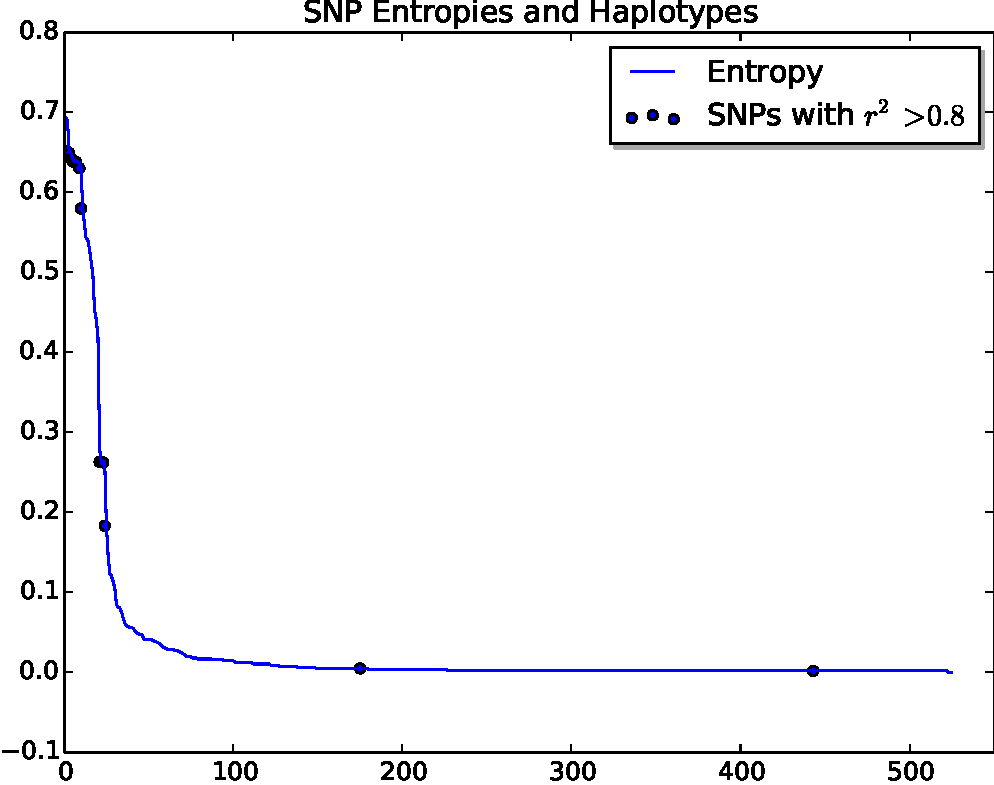
\includegraphics[width=0.7\linewidth]{exon_sorted_entropies_and_haps}
\caption{Entropies of exonic SNPs on BRCA1 and BRCA2 genes, marked with the high-$r^2$ SNPs.}
\label{fig:ents_haps}
\end{figure}

\subsection{Informativeness}\label{sec:inf}
For some SNPs in our datasets, most individuals share the same alleles.
From the perspective of information theory, such SNPs have lower entropies;
they provide less information, and contribute less identifiability of individuals.
These low-entropy SNPs are thus less desirable to keep in the selected set as we reduce the size.
We measure the informativeness of any SNP $d$ in our dataset using the standard metric, Shannon entropy:
\[
H(d) = - \sum_{i}{p_i \log_2(p_i)}
\]
where $p_i$ is the frequency of the $i^{th}$ allele for $d$.
In practice, most SNPs have one major allele, which has a much higher frequency than the other alleles.
The entropies of these SNPs would be low, due to the minor alleles having too low of frequencies,
so we want to select SNPs that have more frequent alleles.
% definition of major and minor alleles, am I using them right?
We compute the entropies of SNPs in our dataset and observe their effects on identifiability,
and we plot their entropies in descending order in Figure \ref{fig:ents_haps}.
We observe that only $7\%$ of the exonic SNPs have entropy values greater than 0.1,
suggesting that there are many that we may be able to exclude from the final selection.

%
\subsection{Linkage Disequilibrium}\label{sec:ld}
% Why is there redundancy? What is LD and what is haplotype?
Studies have found that some SNPs, % what studies?
typically those that locate closely with each other on the genotyping array, tend to be inherited together.
This implies that these SNPs have very similar variability and provide very similar information in terms of identifiability,
and they can hence be considered redundant to all have as our attributes.
Such highly correlated sets of SNPs are termed haplotypes,
and a standard measure of the correlation between SNPs is the correlation coefficient $r^2$,
defined based on the coefficient of $D$.
For alleles $A$ and $B$ with frequencies being $p_A$ and $p_B$, and the frequency of co-occurrence being $p_{AB}$,
\[
D_{AB} = p_A p_B - p_{AB}
\]
\[
{r_{AB}}^2 = \frac{{D_{AB}}^2}{p_A(1-p_A)p_B(1-p_B)}
\]
We use SNP Annotation and Proxy Search (SNAP) \cite{johnson2008snap} to obtain pairwise LD information between SNPs in our dataset and SNPs in their dataset.
Using the pairwise correlation $r^2$ with a threshold of $0.8$, we identify the haplotypes in our dataset, plotted in Figure \ref{fig:ents_haps}.
%This identifies the SNPs that are highly correlated with each other, which are considered redundant and we would aim to exclude from the final set.
According to data from SNAP, our dataset has 3 haplotypes:
one haplotype is located around the $5^{th}$ SNP, one around the $22^{nd}$ and the other on the $176^{th}$ and the $444^{th}$ SNPs.
\\
With the haplotypes determined, we select SNPs in a greedy fashion.
Having the SNPs ranked in a descending order of entropy 
and iterating from the highest-entropy SNP to the lowest,
we select a SNP only if it is not highly correlated with any already selected SNP,
and otherwise we discard it.
This greedy algorithm of SNP selection based on LD allows us to exclude SNPs optimally with respect to information,
as all SNPs solely selected from its haplotype is the one that gives us the most value among all SNPs in that haplotype.
%
%\subsection{Allele Inference with Haplotypes}
%
%
%
%
%
%
%
%
%\section{Current Work}
%.
%\\
%
%
%
%
%
%
%
%
%
\subsection{Solutions}\label{sec:soln}
We propose two solutions to combine the two methods discussed.
One is the simple composition of the two methods, by first removing high-$r^2$ SNPs and then removing low-entropy SNPs.
We apply the two methods in this order so we are able to vary the size of the final selection set and observe the resulted identifiabilities.
We will refer to this solution as the Composition Solution.
\\
The other solution is to regard this problem as a combinatorial optimization problem:
We want to minimize the size of the selected set of SNPs, to maximize the informativeness of the set of SNPs,
and also to reduce the correlation between selected SNPs.
Formally, for a set of $n$ SNPs, where the $i^{th}$ has weight $w_i$ and value $v_i$ and is selected $x_i \in {0, 1}$ times,
the maximum weight of the selection is restricted to be $\leq W$,
and the number of items selected is exactly $C$:
\begin{align*}
\text{maximize}  &\sum\limits_{i=1}^{n}{v_i x_i}\\
\text{subject to } &\sum\limits_{i=1}^{n}{w_i x_i} \leq W \text{,}\\
                           &\sum\limits_{i=1}^{n}{x_i} = C \text{, and}\\
                           &x_i \in {0, 1}
\end{align*}
It is hence an instance of the Knapsack Problem, and we can solve it using the dynamic programming solution.
The weight and value functions are not obvious in our case, but we can define them basing on the entropoy and LD functions.
Below we define $w(d)$ the weight function of a SNP $d$ and $v(d)$ the value function of $d$,
\begin{align*}
w(d) &= \frac{\sum\limits_{p \in \Pi_d} r^2(d, p)}{n}\\
v(d) &= H(d)
\end{align*}
where $\Pi_d$ is the set of proxies of SNP $d$ according to LD data from SNAP, and it depends on the $r^2$ threshold picked.
Note that the weight function is the fraction of SNPs in the dataset that are in a haplotype of size $> 1$,
weighted by the correlation measured in $r^2$, and thus it is normalized to be always between 0 and 1.
And the value function is simply the entropy, as we prefer a SNP more if it has higher entropy.
We will refer to this solution as the Knapsack Solution.
%
%
%
%
\section{Evaluation}
\begin{figure}[t]
    \centering
    \begin{subfigure}{0.45\textwidth}
        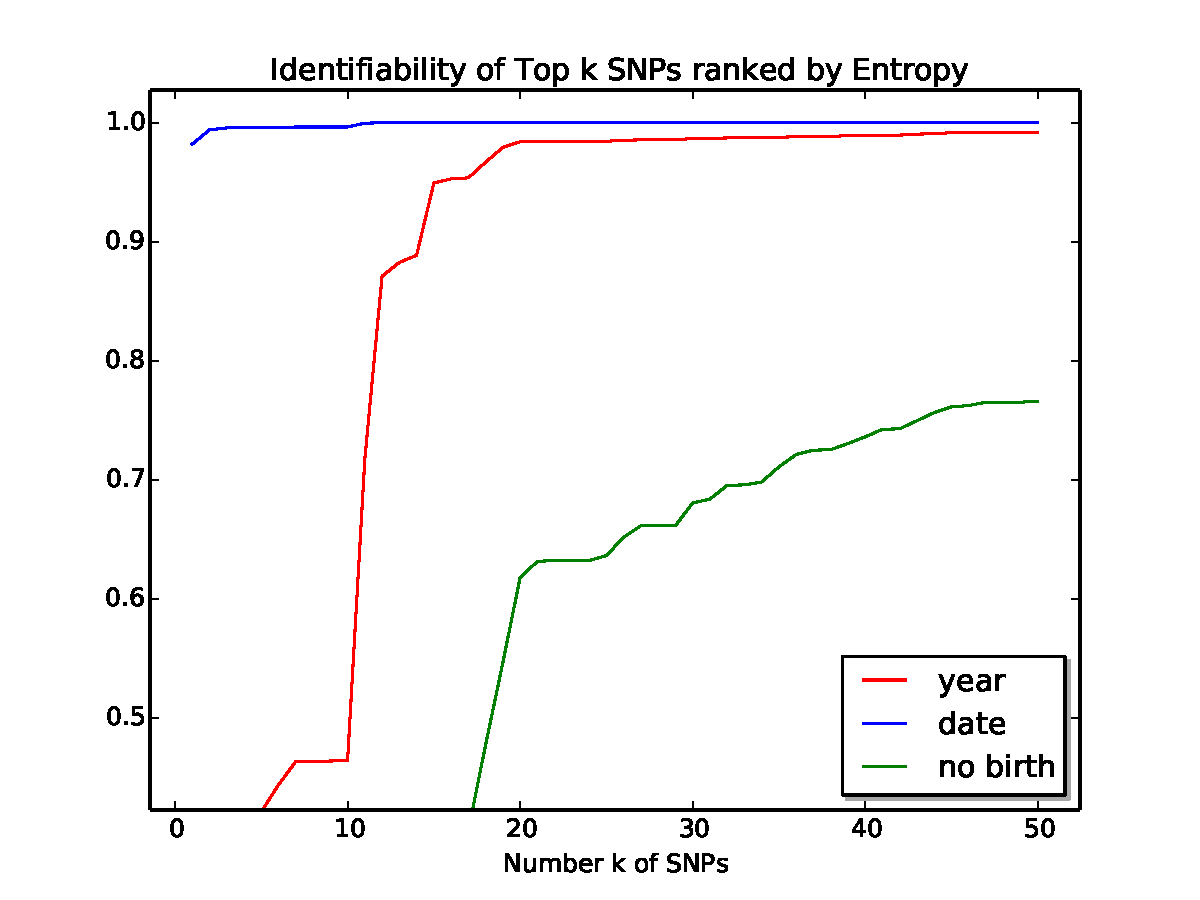
\includegraphics[width=\textwidth]{top_k_entropy}
        \caption{Without high-$r^2$ SNPs removed}
        \label{fig:ent}
    \end{subfigure}
    ~ %add desired spacing between images, e. g. ~, \quad, \qquad, \hfill etc. 
      %(or a blank line to force the subfigure onto a new line)
    \begin{subfigure}{0.45\textwidth}
        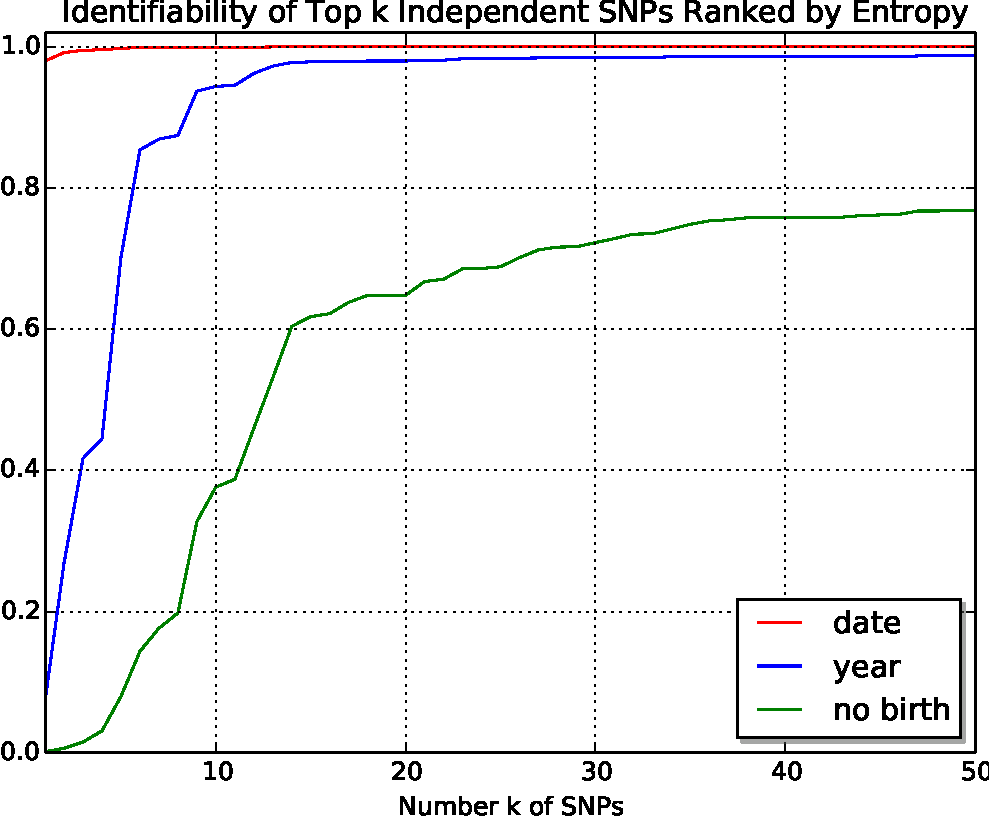
\includegraphics[width=\textwidth]{top_k_entropy_independence}
        \caption{With high-$r^2$ SNPs removed}
        \label{fig:ent_indep}
    \end{subfigure}
    \caption{Identifiability of top $k$ SNPs selected using the Composition Solution.
                  The rate of increase of identifiability reaches the maximum more quickly when high-$r^2$ SNPs have been removed first.}
    \label{fig:topk_ents}
\end{figure}
\begin{figure}[t]
    \centering
    \begin{subfigure}{0.45\textwidth}
        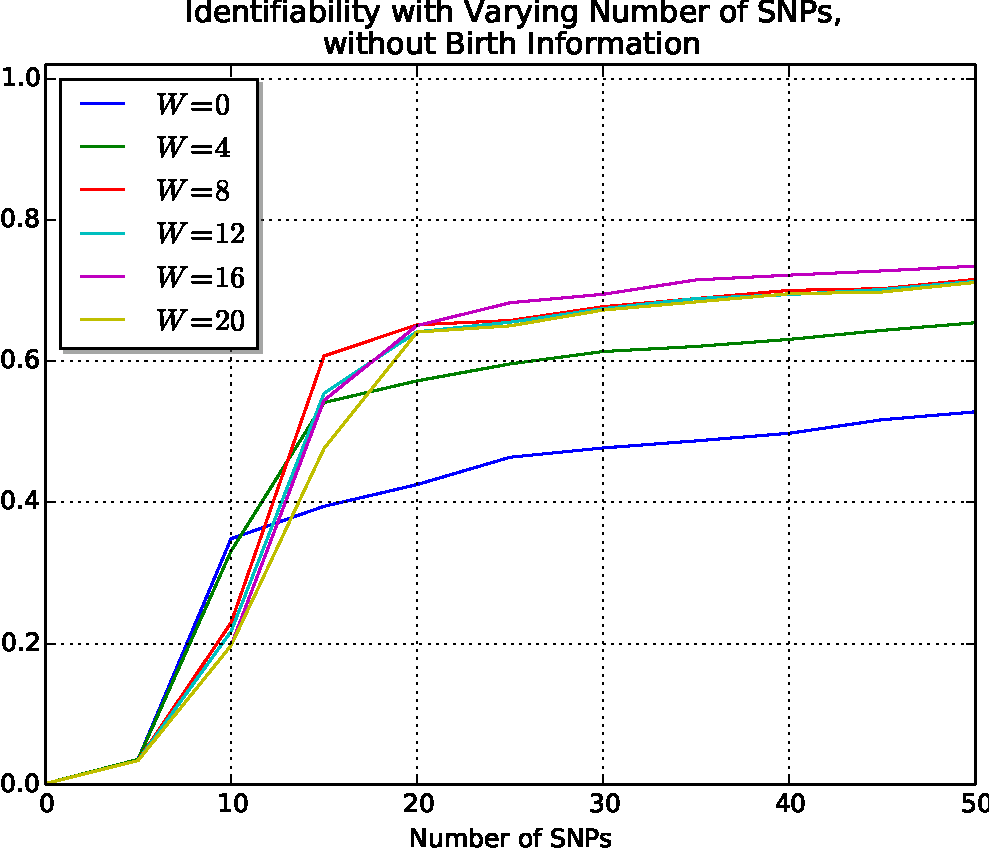
\includegraphics[width=\textwidth]{knapsack_x_C50_W20}
        \caption{With varied maximum weight $W$}
        \label{fig:C50W20}
    \end{subfigure}
    ~ %add desired spacing between images, e. g. ~, \quad, \qquad, \hfill etc. 
      %(or a blank line to force the subfigure onto a new line)
    \begin{subfigure}{0.45\textwidth}
        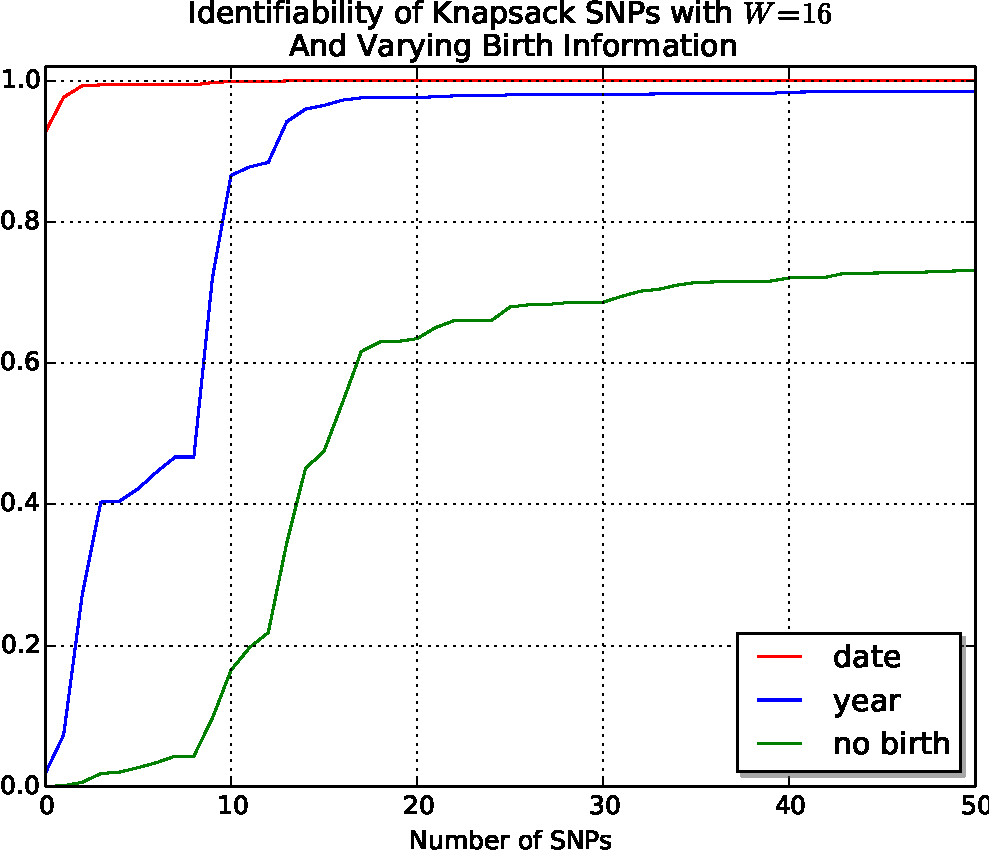
\includegraphics[width=\textwidth]{knapsack_C50_W16_births}
        \caption{With fixed $W$ and varied birth information}
        \label{fig:C50W16births}
    \end{subfigure}
    \caption{Identifiability of top $k$ SNPs selected using the Knapsack Solution.}
    \label{fig:knapsack}
\end{figure}

In this section we present the experiment results of solving the problem using methods and solutions discussed in Section \ref{sec:app_and_soln}.
\subsection{Composition Solution}
In Figure \ref{fig:topk_ents} we show the identifiability of top $k$ SNPs ranked by entropy, where $k$ varies from 0 to 50,
as well as the identifiability of low-$r^2$ (we chose 0.8 as the $r^2$ threshold) SNPs that is ranked and selected in the same fashion.
We also compare the effects of different types of birth information being added in the attributes.
Since we do not have access to the true birth information of the individuals in the 1000 Genome dataset,
we generate synthetic birth information uniformly at random instead.
Naturally, no birth information gives the lowest identifiability, birth year gives better identifiability, and birth date gives the highest.
In particular, we can see that the birth year information is sufficient to give $98\%$ identifiability,
using only $20$ SNPs without the removal of high-$r^2$ SNPs in Figure \ref{fig:ent}.
% and using only $14$ after.
%This is $3.8\%$ and $2.8\%$ of the original set of exonic SNPs.
\\
On the other hand, comparing the high-$r^2$ (dependent) with the low-$r^2$ (independent) SNPs, 
we find that the two plots are similar, since both have the identifiability grow rather quickly as $k$ increases up to some point,
$k=20$ in Figure \ref{fig:ent} and $k=14$ in Figure \ref{fig:ent_indep}, and afterwards start slowing down and converging.
This follows our expectation, as each excluded dependent SNP does not provide more information than its selected counterpart,
and identifiability is not affect much by including it in the selection and increasing the size of the selection.
Indeed, we observe a deceleration of growth in Figure \ref{fig:ent} between $k=2$ and $k=10$.
Such deceleration is unobserved in Figure \ref{fig:ent_indep}, and the number of SNPs required to reach $98\%$ identifiability is significantly reduced.
%
%
%
%
\subsection{Knapsack Solution}
For the Knapsack formulation of the problem, since there is not an intuitive way of interpreting and setting the maximum weight $W$ of a selection,
we normalize the weights to have a sum of $100$.
In Figure \ref{fig:C50W20} we fix birth information to use none of it, and we vary the number of SNPs selected
and plot $W$ from $0$ to $20$ to observe the effect on identifiability of different choices of $W$.
The identifiabilities are very similar for $W=8, 12, 16, 20$, and in particular $W=16$ gives the highest.
In Figure \ref{fig:C50W16births} we compare effects of varied amount of birth information, fixing $W$ at $16$ as it produced the best results.
\\
We see a similar trend where the rate of growth of identifiability is high at the start and becomes low after a point, when the number of SNPs is $18$.
This is similar to what we saw in Figure \ref{fig:ent_indep}, but the transition point comes later.
We also observe that without birth information,
the highest identifiability of the Knapsack Solution is lower than the Composition Solution (both using $50$ SNPs) by $5\%$.
Moreover, we observe the same deceleration of the growth rate of the identifiability within the first $10$ SNPs, as we did in Figure \ref{fig:topk_ents},
and we notice that the deceleration is shorter than \ref{fig:ent} but longer than \ref{fig:ent_indep}.
Though better than using the entropy method alone, our Knapsack Solution produces slightly worse results than the Composition Solution.
%
%
%
%
%
\section{Conclusion and Future Work}
In this study we explore identifying of overlapping individuals among different sources of data,
using genotype attributes as well as personal attributes, namely SNPs and birth information.
We develop two methods to exclude less desirable SNPs, based on entropy and LD information.
To combine these two methods to produce resulting selections of SNPs we also develop two solutions:
one is a simple composition of the two methods,
and the other is defining a Knapsack problem where the weight function is based on the LD information and the value function on entropy.
We compare the efficacy of these two solutions, and we find that the Composition Solution produces selections of SNPs that have higher identifiabilities.
In conclusion, we are able select $17$ SNPs out of the $525$ exonic BRCA1 and BRCA2 SNPs
and achieve identifiability $98\%$ with birth year information, using the Composition Solution.
\\
Following is a complete comparison of the minimum amount of SNPs that each solution requires
to reach a certain amount of identifiability for each type of birth information.
We choose different identifiability thresholds here as they converge differently across different birth types.
For each birth type, to reach the chosen identifiability, the Composition Solution always requires fewer SNPs than the Knapsack Solution.
\begin{center}
  \begin{tabular}{ | r | c | c |}
    \hline
                           & Composition & Knapsack \\ \hline
    Date -- 100\% & 12 & 13 \\ \hline
    Year -- 98\%   & 17 & 25 \\ \hline
    None -- 60\%  & 13 & 17 \\
    \hline
  \end{tabular}
\end{center}
Nevertheless, the definitions of weight and value functions we adopted in this work are rather preliminary,
and there may be more potential to the Knapsack Solution that we may want to explore.
For example, the current formulation of the Knapsack problem depreciates SNPs that are in a larger haplotype.
This results in an unfair preference over SNPs with similar values but belong to smaller haplotypes.
It also only account for LD above the selected $r^2$ threshold and loses more granular LD information.
More importantly, the current formulation of the Knapsack problem assumes independence between an item and the selection made in the computation of weight,
and this is not the case for our setting.
Instead, we should weigh SNPs within a haplotype differently according to their value,
so once the highest-value SNP in the haplotype is selected, the remaining are increasingly unlikely to be selected.
In addition, in this study we focused on one dataset of SNAP and one $r^2$ threshold.
We may want to explore other thresholds of $r^2$ and SNAP datasets for determining haplotypes.
%
%
%
%
%
%    
%
%
%
%
%
%
% 
%
%
%
%
%
%
%
%
%
%
%
%
%
%
%
%
\bibliographystyle{plain}
\bibliography{cryptohash_writeup}
%
\end{document}  




























